\chapter{Experiments and results}

We evaluate the metric learning method described in this thesis in two ways. Firstly, we evaluate how well the learned metric approximates the target metric. In other words, how well does the method align feature space to the structured output space? This can be measured by the \acf{MSE} between the learned distances in feature space and the loss in output space. Secondly, we evaluate how much the learned metric improves performance over the default Euclidean metric on the overall prediction task. We do this by measuring the task-specific performance of a \ac{kNN} classifier using the learned metric and see if this improves over the Euclidean metric. We compare both these results against a baseline metric learning algorithm that uses binary similarity constraints, namely the ITML algorithm. \cite{davis2007information}

We run these evaluations on two datasets taken from structured prediction problems. The first dataset comes from an attribute-based classification problem, while the second comes from a semantic segmentation problem. Both these datasets have a real-valued loss defined on the structured output space. This real-valued loss allows us to test the idea of aligning the feature space to the output space through metric alignment by using the loss function as the target metric.



\section{Datasets}
%datasets, learning problems, features, ground-truth, loss functions, classes, number of instances


\subsection{Attribute-based classification dataset}

Attribute-based classification is an approach to object recognition which can be applied to problems where there is no training data for the test categories. This problem is known as zero-shot or zero-data learning. In attribute-based classification, classes are described by high-level ``semantic'' attributes. These attributes are properties of an object for which a human can decide whether this property applies to the object. In this way, previously unseen classes can be described by its attributes. By learning the connection between visual features and attributes a classifier can correctly classify members of these unseen classes. 

For our evaluation we use the \acf{AwA} dataset\footnote{Available at \url{http://attributes.kyb.tuebingen.mpg.de/}.} described in \cite{lampert2009learning, lampert2014attribute}. This dataset contains images of 50 different species of mammals. A set of 85 semantic attributes describes each class and the class-attributes table is available in both a continuous-valued matrix as well as a binary one obtained by thresholding at the mean value.

\subsubsection{Image features}

Several pre-computed features are distributed along with the \ac{AwA} set in order to promote repeatability of experiments done using the dataset. We make use of the SURF histogram features. \emph{Speeded up robust features} (SURF), originally presented in \cite{bay2006surf}, are scale and rotation invariant image features that are similar to the well-known SIFT feature. \cite{lowe2004distinctive} Scale-invariant interest points are detected by finding locally maximal response to an approximate Hessian filter on the lightness values of an image. This gives comparable performance to the Harris-Laplace detector used in SIFT, but because the approximation to the Hessian can be computed from integral images it is faster to compute. A dominant orientation is estimated for each point using Haar-wavelet responses which are also cheap to compute using integral images. The descriptor itself user Haar-wavelets as well: it sums responses to a vertical and horizontal wavelet for a local neighborhood in a $4 \times 4$ grid.

The SURF-histogram feature used to describe each image in the \ac{AwA} set is visual bag of word (BoW) approach to classification based on these SURF features. A visual codebook is created by clustering the SURF features computed from the dataset using the $k$-means clustering algorithm. Each cluster centroid in descriptor space is then taken as a visual word. The feature vector for a specific image is then formed by computing the SURF descriptors for the image, assigning each descriptor to the closest cluster centroid and creating a histogram of these assignments. The pre-computed features use a codebook of 2000 visual words.

We pre-process these features by first L1 normalizing them. Then we standardize them by subtracting the mean and dividing by the standard deviation. This ensure the data has zero-mean and unit-variance. We further reduce the dimensionality to 128 dimensions using the principal component analysis algorithm in order to make the computations more tractable.

\subsubsection{Target metric and constraints}

In order to generate the constraints on which we train the metric learning algorithm we sample $100 n$ random pairs of points without replacement, where $n$ is the number of feature vectors in the training set. These pairs form the set $\mathcal{A}$ on which our absolute distance constraints are defined. The absolute distance constraints are formed by choosing a target metric and calculating its value for each of the sampled pairs in $\mathcal{A}$. For the \ac{AwA} set we choose Hamming distance between the attribute vectors corresponding to the classes of the images in the pair.   The Hamming distance is calculated as:
\begin{align}
d_{\text{H}}(i, j) &= \|\vec{a}_i - \vec{a}_j\|_{\text{H}}, \\
 &= \sum_{k=1}^{n} \left[ a_{i,k} = a_{j,k} \right],
\end{align}
where $(\vec{x}_i, \vec{x}_j)$ is one of the sampled pairs in $\mathcal{A}$ and $\vec{a}_i$ and $\vec{a}_j$ are the corresponding attribute vectors consisting of $n$ binary attribute values $a_{i,k}$. Further $[ \cdot ]$ denote Iverson brackets which take the value 1 if the enclosed equation evaluates as true. The absolute distance constraints are expressed as:
\begin{align}
d_{\mat{A}}(\vec{x}_i, \vec{x}_j) &= d_{\text{H}}(i, j) & (i, j) &\in \mathcal{A},
\end{align}
where $d_{\mat{A}}(\vec{x}_i, \vec{x}_j)$ is the metric distance being learned by our metric alignment algorithm.

In order to train our baseline metric learning algorithm we also need a set of binary similarity constraints. Since each image in the \ac{AwA} set is assigned to single class, these are easy to generate by constraining the distance between pairs of the same class to be small and pairs of differing classes to be large. We thus divide our sampled pairs $(i,j) \in \mathcal{A}$ into two disjoint sets $\mathcal{S}$ and $\mathcal{D}$ for similar and dissimilar classes respectively. The constraints are defined as:
\begin{align}
d_{\mat{A}}(\vec{x}_i, \vec{x}_j) &\leq u & (i, j) &\in \mathcal{S}, \\
d_{\mat{A}}(\vec{x}_i, \vec{x}_j) &\geq \ell & (i, j) &\in \mathcal{D},
\end{align}
where we set $u$ and $l$ to be the $5^{th}$ and $95^{th}$ percentile of the distribution of distances on a small subset of 5000 pairs sampled from the training set.

\subsubsection{Task description}

We use the \ac{AwA} set in the context of two learning problems: a standard multiclass classification problem and a zero-shot learning problem as described in \cite{lampert2014attribute}. For the multiclass task we randomly divide the images 50/50 into a training and a test set while keeping the distribution among classes the same. We then learn our metric on the training set using the constraint described above. Next we classify the test images using a $k$-nearest neighbor classifier. The parameter $k$ is tuned by 2-fold cross validation on the training set using the Euclidean metric, and was set to $k = 50$.

In zero-shot learning, the classes in the dataset are split, such that the set of classes in the train set is disjoint from the set of classes in the test set. Therefore, this task can not be solved using a regular $k$-NN classifier. Lampert et al. describe two different approaches to  attribute based classification for zero-shot learning: \emph{direct attribute prediction} and \emph{indirect attribute prediction}. For simplicity we will constrain ourselves to the direct attribute prediction method. In this method  a probabilistic classifier is learned that predicts the probability $p(a | \vec{x})$: the probability for an attribute value $a$ given the image feature $\vec{x}$. We calculate this probability by finding the $k$-nearest neighbors of the feature vector and calculating the proportion that take the same attribute value:
\begin{equation}
p(a | \vec{x}) = \frac{1}{k} \sum_{i=1}^{k} \left[a^i = a\right].
\end{equation}
Here $a^i$ is the value for the attribute of the $i^th$ nearest neighbor and $[\cdot]$ denotes the Iverson brackets. Using these probabilities the test class $z$ is found through MAP prediction assuming independent attributes:
\begin{equation}
h(\vec{x}) = \argmax_{z \in \mathcal{Z}} \prod_{m=1}^{M}\frac{p(a^{z}_m | \vec{x})}{p(a^{z}_m)},
\end{equation}
where $\mathcal{Z}$ is the set of unseen test classes, $a^z_m$ is the $m^th$ element of the attribute vector for class $z$ and $\vec{x}$ is the input feature. We calculate $p(a^{z}_m | \vec{x})$ using the $k$ nearest neighbors and we calculate the prior $p(a^{z}_m)$ as the proportion of training classes having attribute value $a^{z}_m$.



\subsection{Semantic segmentation dataset}

Semantic segmentation is a computer vision problem in which the objective is to segment input images into contiguous regions by assigning labels to each pixel. The labels are drawn from a predefined set of object and background class labels. Annotations for the training set are often provided by hand and usually not all pixels receive a label in these annotations.

For our evaluation we use the \acf{MSRCv1} dataset.\footnote{The MSRC datasets are available at \url{http://research.microsoft.com/en-us/projects/objectclassrecognition/}.} The \ac{MSRCv1} set consists of 240 images, segmented into 9 classes. The images are loosely segmented, meaning that the annotations are not pixel-perfect. The segmentations cover most of each image with some of the pixels not having a label. The 9 classes contain both foreground object classes, e.g. car, cow, face, and background classes, e.g. grass, sky. There is limited variation in appearance and scene within each class as the pictures have been taken in the same manner, often around the same location.

\subsubsection{Image features}

For the \ac{MSRCv1} set we use CSIFT color descriptor. \cite{abdel2006csift} The CSIFT descriptor is calculated the same as regular SIFT descriptors, but instead of calculating it on the gray-scale image, a SIFT descriptor is calculated on the three channels of a color invariance model presented in \cite{geusebroek2001color}. We calculate the CSIFT descriptors using the color descriptor software from \cite{sande2011empowering}.  From each training image we extract feature vectors $\vec{x}$ on a regular hexagonal grid $(\vec{u}, \vec{v})$, with $\vec{x}$ computed from the image area centered on image coordinates $(u_i, v_i)$. Each of these feature vectors $\vec{x}_i$ is paired to a label patch $\vec{y}$ taken from the training annotation for the image and centered at $(u_i, v_i)$. We again normalize and standardize these features and reduce the dimensionality to 128 dimensions using principal component analysis.

\subsubsection{Target metric and constraints}

For the \ac{MSRCv1} set, the target metric we use for the constraints is the segmentation overlap. This is given as the proportion of overlapping pixel labels between the segmentation patches corresponding to the image patches in the pair $(i,j)$ and is calculated as:
\begin{align}
d_{\text{P}}(i, j) &= 1 - \text{Acc}(\vec{y}_i, \vec{y}_j) \\
&= 1 - \frac{ \sum_{k=1}^{n} \left[ y_{i,k} = y_{j,k} \right] }{ \sum_{k=1}^{n} \left[ y_{i,k} \in \mathcal{L} \wedge y_{j,k} \in \mathcal{L} \right]},
\end{align}
where $\vec{y}_i$ is the segmentation patch corresponding to the image patch represented by the feature vector $\vec{x}_i$. This patch consists of $n$ elements, here indexed by $k$, and $\mathcal{L}$ denotes the set of possible labels. This measure counts the number of pixels that have the same label as a proportion of the number of pixels that have been labeled in both patches, and subtracts this from one to turn it into a distance function.

Because the majority of patches does not overlap at all, we do not sample the pairs globally as we do with the \ac{AwA} set. Instead, for each point in the training set we find the 100 nearest neighbors and use these neighbor pairs as the set $\mathcal{A}$ for our constraints. These constraints are thus given as:
\begin{align}
d_{\mat{A}}(\vec{x}_i, \vec{x}_j) &= d_{\text{P}}(i, j) & (i, j) &\in \mathcal{A},
\end{align}

Since the label patches are not assigned to a single class, we cannot generate binary similarity constraints based on class assignment. Instead, we threshold the target metric $d_{\text{P}}$. Because $d_{\text{P}}$ ranges from 0 to 1 we set the threshold at 0.5:
\begin{align}
d_{\mat{A}}(\vec{x}_i, \vec{x}_j) &\leq u & \text{if} \quad d_{\text{P}}(i, j) < 0.5, \\
d_{\mat{A}}(\vec{x}_i, \vec{x}_j) &\geq \ell & \text{if}  \quad d_{\text{P}}(i, j) \geq 0.5.
\end{align}
Again we set $u$,$l$ to be the $5^{th}$ and $95^{th}$ percentile of the distances distribution over a sample of pairs from the train set.

\subsubsection{Task description}

Segmentation benchmarks consist of images $\mat{I}$ where each pixel $\mat{I}_{(u,v)}$ is usually given as a triple $(r,g,b)$ denoting the color of a single pixel and segmentations $\mat{S}$ of which each element  $\mat{S}_{(u,v)} \in \mathcal{Y}$ assigns a label to pixel $\mat{I}_{(u,v)}$ of the image. Here $\mathcal{Y} = \{1, 2, \ldots, n\}$ is a predetermined label set  where each label corresponds to one of $n$ visual classes. 

We randomly divide the images of each data set 50/50 between a training set and test set. In order to keep the class distribution for each subset similar we split the \ac{MSRCv1} set per image sequence, since each sequence of photographs was taken in a single context and thus shows a similar distribution of classes.

For our dataset we extract square patches from the images and the corresponding segmentations. The task is then to create the correct label patch $\vec{y}$ given a test feature vector $\vec{x}$ extracted from the image patch. We do this by finding the $k$-nearest neighbors of the feature vector among the training set and combining the corresponding $k$ label patches by majority voting for each pixel separately. The parameter $k$ is tuned by 2-fold cross validation on the training set using the Euclidean metric, and was set to $k = 10$.



\section{Metric alignment experiment}

The first experiment is designed to test how well the metric learning method presented in this thesis can approximate the given target metric, with the target metric being the loss function for the learning problem at hand. If the learned distance in feature space is closely aligned to the loss, this means that the space is well-clustered: small distances in feature space correspond to small loss between the corresponding output structures. This is beneficial for prediction algorithms making predictions in this feature space, an effect which we will evaluate in the next experiment. 

We quantify the alignment between the learned metric and the target metric in the form of a squared prediction error, namely the mean squared error between the distances calculated according to the learned metric and the target metric.  We evaluate this on a sample of pairs from the test set, sampled in the same way as the training pairs, either globally or locally. Our \ac{MSE} evaluation measure on the test set is thus calculated as:
\begin{equation}
\text{MSE}_{\mathcal{T}}(d_{\mat{A}}, \hat{d}) = 
\frac{1}{|\mathcal{T}|}\sum_{(i,j) \in \mathcal{T}} \left(d_{\mat{A}}(\vec{x}_i, \vec{x}_j) - \hat{d}(i, j)\right)^2.
\end{equation} 
Here $d_{\mat{A}}$ is the learned metric and $\hat{d}$ is the target metric, either $d_{\text{H}}$ for the \ac{AwA} set or $d_{\text{P}}$ for the \ac{MSRCv1} set. The set $\mathcal{T}$ of pairs $(i,j)$ is the sample of pairs from the test set.

We compare the metric learned by our algorithm against two baselines. Firstly, the Euclidean metric, given by $\mat{A} = \mat{I}$. Secondly, against a metric learned by \acf{ITML}. \cite{davis2007information} While the metric alignment method is trained using the absolute distance constraints, \ac{ITML} is trained using the binary similarity constraints.


\subsection{Results}

For our alignment test we train metric alignment on the absolute distance constraints for both the AwA and the MSRCv1 datasets and compare this against the Euclidean metric and against a metric learned by the ITML algorithm on binary similarity/dissimilarity constraints. For each dataset we sample $100n$ pairs from the test set, where $n$ is the number of points in the test set. We evaluate the mean squared error (MSE) between the learned metric distance between the feature vectors and the target metric distance.

\begin{table}
\begin{center}
\caption{Mean square error (MSE) between learned metric distance and target metric distance on test sets.}
\label{tab:alignment}
\begin{tabular}{lcc}
\toprule
& \multicolumn{2}{c}{Dataset} \\
 Metric & AwA & MSRCv1 \\
\midrule
Euclidean & 303.86 & 279.49 \\
ITML & 302.55 & 279.46 \\
Metric Alignment & 114.00 & 279.00 \\
\bottomrule
\end{tabular}
\end{center}
\end{table}

Table \ref{tab:alignment} presents our results. It shows that for the AwA dataset, metric alignment reduces the MSE compared to both the Euclidean metric and the ITML algorithm. However, for the MSRCv1 dataset this effect is negligible. Furthermore, the alignment between the learned metric and the target metric still leaves a considerable error term, showing that the alignment is not complete.

These results show that the metric alignment method is at least able to move the metric on the feature space towards the target metric in the output space and that this alignment is closer in terms of MSE on at least one dataset than that between the original feature space and the target metric and closer than a metric learned by the ITML algorithm on binary similarity constraints and the target metric.


\section{Structured prediction experiment}

Our second experiment tests the effect of metric alignment on the ability of a \acf{kNN} classifier to predict the correct output. \ac{kNN} is a non-parametric classification method, which means that its decision function is not characterized by a parameterized model. Instead, the class for an input point is decided to be the majority class amongst the most similar points in the training set, the nearest neighbors. Although it requires storing of the whole training set, which may become problematic for large sets, the \ac{kNN} classification method is simple, requires little parameter tuning and is inherently applicable to multi-class problems. The \ac{kNN} classifier depends on nearest neighbors having low loss relative to the ground truth output, thus learning a metric with the loss as target metric should improve prediction performance.

We implement our \ac{kNN} algorithm using \ac{FLANN}. \cite{muja2009fast} The training features are stored in a set of randomized kd-trees. This allows for fast and parallel retrieval of nearest neighbors. We set the \ac{FLANN} parameters to create 4 trees and check a maximum of 1024 leafs during retrieval.

We evaluate this experiment on the prediction accuracy. We calculate the normalized multiclass accuracy, which is the mean of the true positive rates of each class:
\begin{equation}
Acc = \frac{1}{|\mathcal{Z}|} \sum_{z \in \mathcal{Z}} \frac{\text{TP}_z}{\text{TP}_z + \text{FN}_z}.
\end{equation}
Here $\mathcal{Z}$ is the set of all test classes: all classes for the multiclass and segmentation tasks, but only the hidden classes for the zero-shot task. Further, $\text{TP}_z$ and $\text{FN}_z$ denote the true positives respectively false negatives for class $z \in \mathcal{Z}$. Again, we evaluate these measures against the same baselines as in the metric alignment experiment: Euclidean metric and \ac{ITML}.


\subsection{Results}

For our classification accuracy test we use a $k$NN algorithm to solve the AwA multiclass classification and zero-shot learning tasks and the MSRCv1 patch segmentation tasks. The neighbors are sought using the original Euclidean feature space, using a metric learned by the ITML algorithm on binary similarity/dissimilarity constraints, and using our metric alignment algorithm on the absolute distance constraints generated using the target metric.

For testing we sample $100n$ pairs from each test set, where $n$ is the number of points in the test set. We evaluate the mean class accuracy of the predicted classes or segmentations. The results are displayed in Table \ref{tab:accuracy}.

\begin{table}
\begin{center}
\caption{Mean class accuracy on the AwA multiclass and zero-shot tasks and MSRCv1 patch segmentation task.}
\label{tab:accuracy}
\begin{tabular}{lccc}
\toprule
& \multicolumn{3}{c}{Dataset} \\
& \multicolumn{2}{c}{AwA} & MSRCv1 \\
\cline{2-3}
 Metric & multiclass & zero-shot &  \\
\midrule
Euclidean & 0.129 & 0.252 & 0.368 \\
ITML & 0.128 & 0.251 & 0.368 \\
Metric Alignment & 0.114 & 0.210 & 0.368 \\
\bottomrule
\end{tabular}
\end{center}
\end{table}

These results clearly show that while the metric learned using the ITML algorithm has no impact on the prediction accuracy, the metric learned using the metric alignment algorithm has a negative effect on the prediction accuracy for the AwA dataset. This is the same set on which the MSE measuring the alignment improved the most.


\section{Analysis}

In order to resolve the apparent contradiction between the alignment results as measured by MSE on the fit of the learned metric to the target metric and by the prediction accuracy as measured by the mean class accuracy, we take a closer look at what exactly it is that our metric learning algorithm is learning in the alignment experiment.

\begin{table}
\begin{center}
\caption{Pearson correlation (Pearson r) between learned metric distances and target metric distances on the test sets.}
\label{tab:pearson}
\begin{tabular}{lcc}
\toprule
& \multicolumn{2}{c}{Dataset} \\
 Metric & AwA & MSRCv1 \\
\midrule
Euclidean & 0.124 & 0.166 \\
ITML & 0.126 & 0.166 \\
Metric Alignment & 0.100 & 0.165 \\
\bottomrule
\end{tabular}
\end{center}
\end{table}

Firstly, we look at the Pearson correlation statistic between the learned metric distances and the target metric distances for the sample pairs taken from the test sets. This statistic measures the linear correlation between the two sets of measurements. In other words, this measures the proportionality between the learned metric distance and the target distance. This is exactly the alignment we are trying to achieve through metric learning. It ranges between 1 and -1, with 1 being exact linear correlation, -1 being inverse linear correlation and 0 being no linear correlation. The results are shown in Table \ref{tab:pearson}.

The Pearson correlation results show that our metric alignment algorithm markedly \emph{reduces} the correlation between the learned metric and the target metric. Thus the MSE decreases, since that is the measure that we minimize in our algorithm, but the alignment decreases as well. This is also shown in Figure \ref{fig:alignment}. Here we plot the learned metric distances along against the target distances. The learned distances are plotted along the y-axis, scaled to be between 0 and 1, and the target distances are plotted along the x-axis, also scaled.Testing pairs are shown as a white scatter plot, with the density visualized as a color jet with blue being low density and dark red being highest density. Also shown is the diagonal. The more points lying along the diagonal, the better the alignment. The plot for metric alignment seems to show that the distances get squashed in a narrower range of learned distances. This hurts the alignment.

One possible reason why this might happen has to do with our choice for a squared error measure. Since it is squared, this is very vulnerable to outliers. Because of our high-dimensional features there can easily be many pairs with a large distance between them in feature space. This is shown in the scatter plot by the outliers on the top half of the plot and the tendency of the metric learning algorithm to squash these values into a more narrow range. 

\begin{figure}[p]
\begin{subfigure}{.5\textwidth}
  \centering
  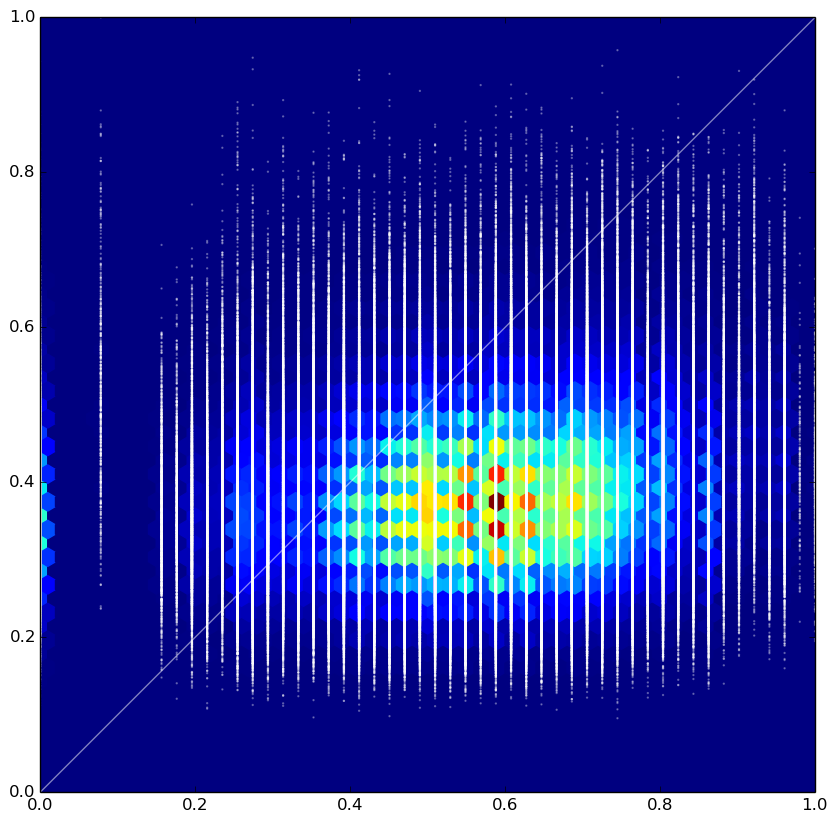
\includegraphics[width=\textwidth]{Figures/Euclidean_Metric_test_AwA}
  \caption{Euclidean AwA}
  \label{fig:sub1}
\end{subfigure}%
\begin{subfigure}{.5\textwidth}
  \centering
  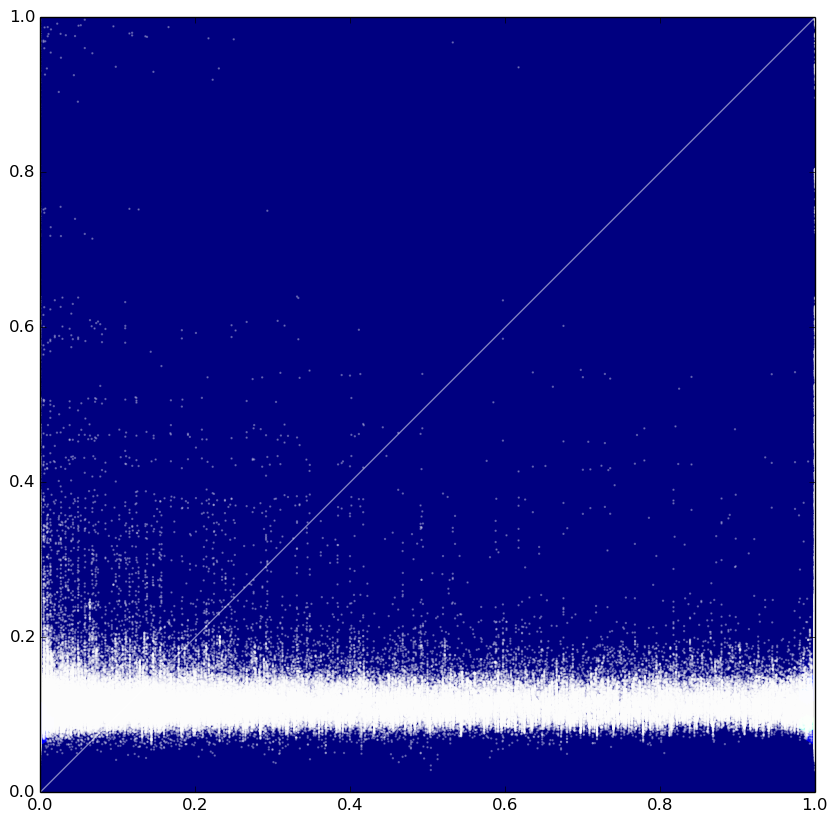
\includegraphics[width=\textwidth]{Figures/Euclidean_Metric_test_MSRCv1}
  \caption{Euclidean MSRCv1}
  \label{fig:sub2}
\end{subfigure}
\begin{subfigure}{.5\textwidth}
  \centering
  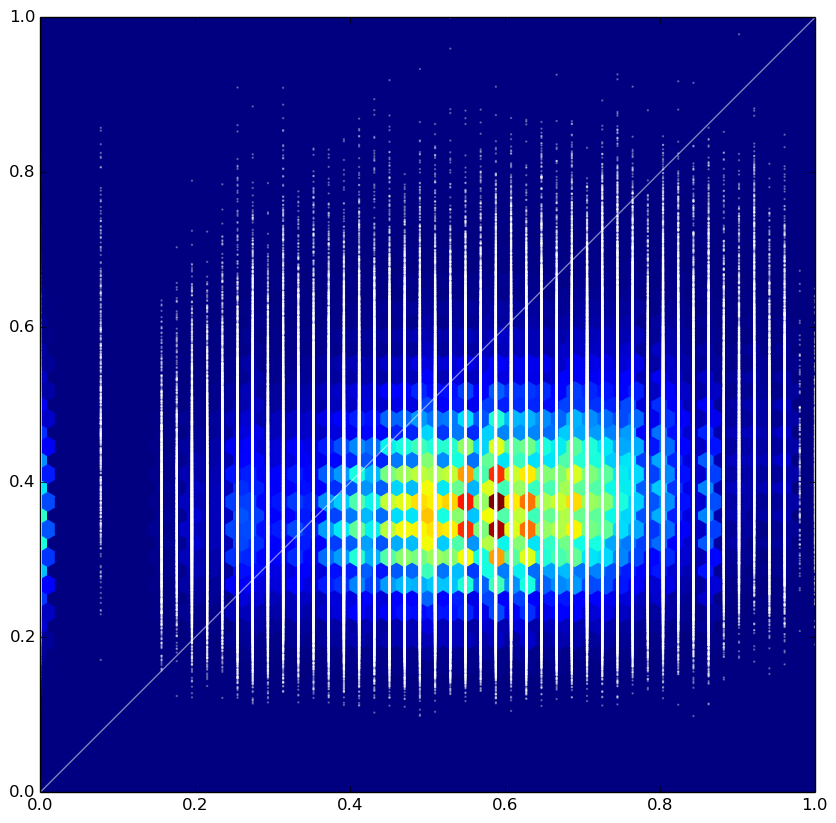
\includegraphics[width=\textwidth]{Figures/ITML_test_AwA}
  \caption{ITML AwA}
  \label{fig:sub3}
\end{subfigure}%
\begin{subfigure}{.5\textwidth}
  \centering
  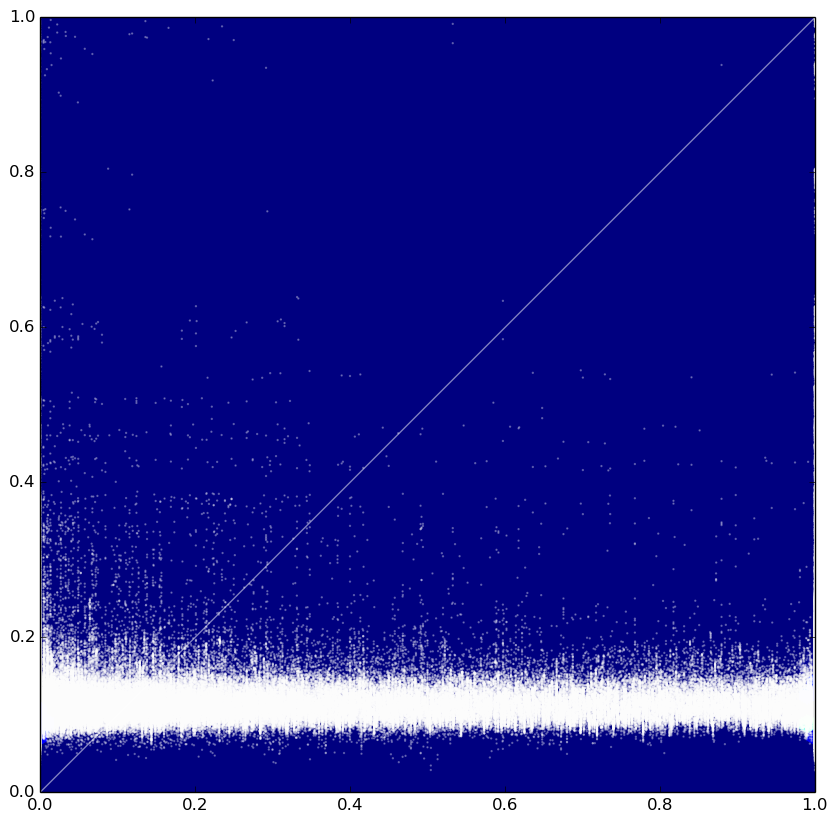
\includegraphics[width=\textwidth]{Figures/ITML_test_MSRCv1}
  \caption{ITML MSRCv1}
  \label{fig:sub4}
\end{subfigure}
\begin{subfigure}{.5\textwidth}
  \centering
  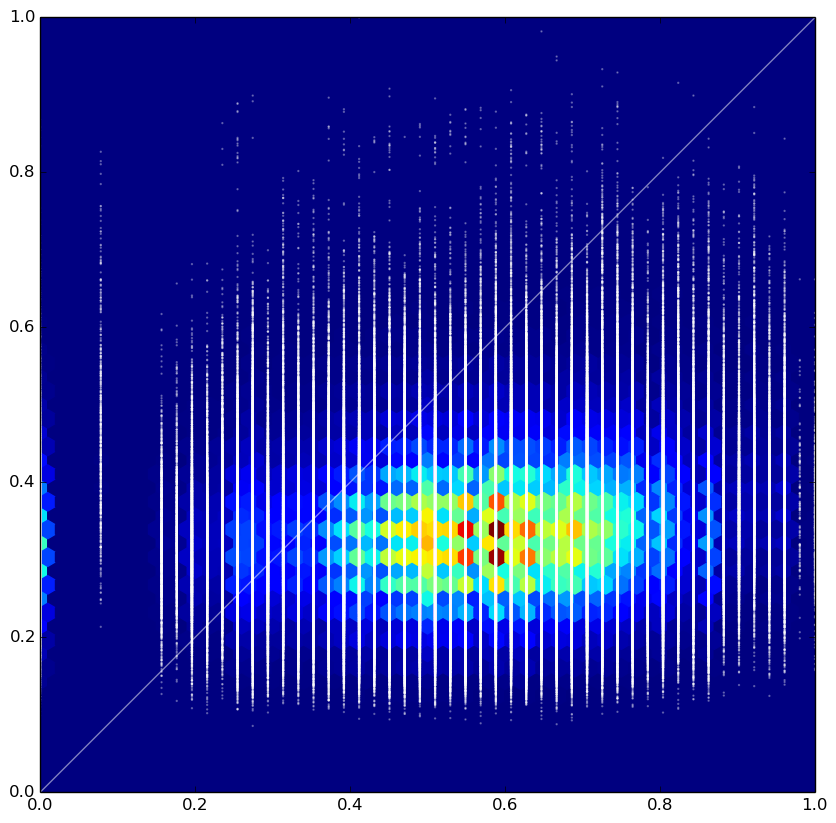
\includegraphics[width=\textwidth]{Figures/Metric_Alignment_test_AwA}
  \caption{Metric Alignment AwA}
  \label{fig:sub5}
\end{subfigure}%
\begin{subfigure}{.5\textwidth}
  \centering
  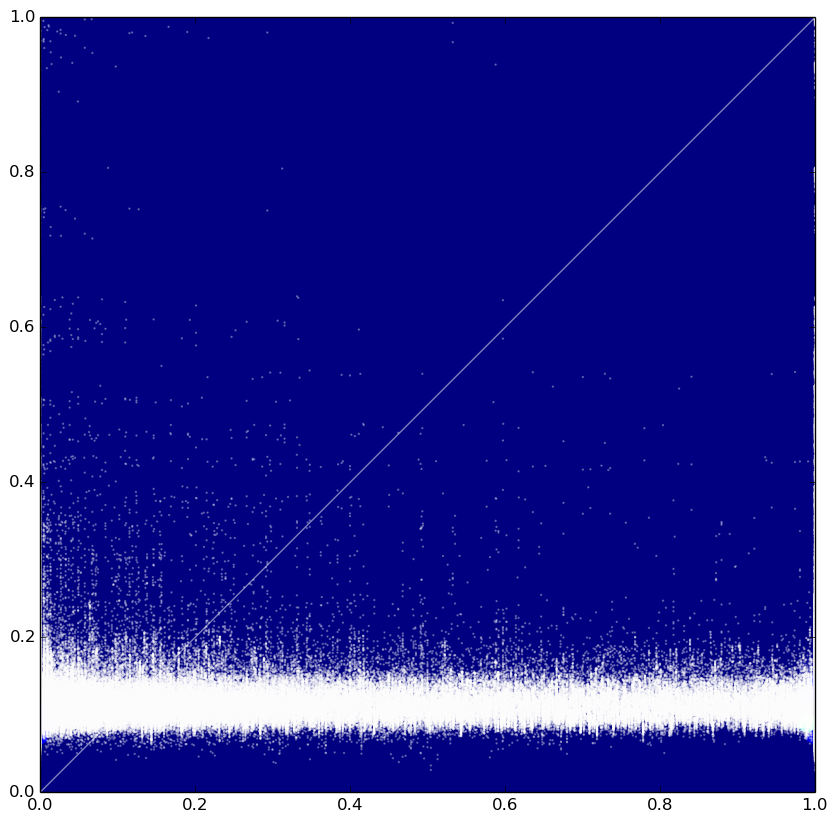
\includegraphics[width=\textwidth]{Figures/Metric_Alignment_test_MSRCv1}
  \caption{Metric Alignment MSRCv1}
  \label{fig:sub6}
\end{subfigure}
\caption{Plots showing the alignment between learned and target distances. The learned distances are plotted along the y-axis, scaled to be between 0 and 1, and the target distances are plotted along the x-axis, also scaled. Testing pairs are shown as a white scatter plot, with the density visualized as a color jet with blue being low density and dark red being highest density. Also shown is the diagonal.}
\label{fig:alignment}
\end{figure}































